%!TEX root = ../3dchapter.tex
% chktex-file 46
% chktex-file 36

\setchapterpreamble[u]{\margintoc}

\graphicspath{{conversion/}}
\renewcommand*{\thelesson}{6.2}

\chapter{Conversions between 3D representations and formats}%
\label{chap:conversion}

This lesson describes different conversions between 3D representations and formats that a geomatics engineer might have to perform.
It does not claim to be an overview of all potential conversions, but it rather offers insights about the algorithms and methods most commonly used, and points out pitfalls to be aware of.

%

The lesson is divided into two distinct parts:
\begin{description}
  \item[Fields:] conversions that are performed when we are dealing with a \emph{field}, let it be the temperature or the concentration of a certain chemical in the air (modelled as a 3D volume).
  We name such field a trivariate field: each location ($x,y,z$) in space has one attribute.
  \index{trivariate field}\marginnote{trivariate field}
  Voxels are usually what is used to represent, exchange, and analyse fields in 3D.
  \index{voxels}\marginnote{voxels}
  \item[Objects:] when we are dealing with data (points, surfaces, and volumes) that represent the boundaries of objects in our environment. 
  These can be sample points from lidar or dense matching of images, or the b-rep of some buildings (which have been reconstructed with different acquisition methods).
  \index{b-rep}\marginnote{boundary representation (b-rep)}
\end{description}

\begin{kaobox}[frametitle=\faExternalLink\ To read or to watch.]
  The reader is advised to first read the two chapters about spatial interpolation (Chapters~4 and 5) in the book \emph{Computational modelling of terrains}~\citep{terrain_book}, where the 2D concepts are introduced.
\end{kaobox}



%%%
%
\section{Conversions for fields}


A field is a model of the spatial variation of an attribute $a$ over a spatial domain, we assume this domain to be $\mathbb{R}^d$, the $d$-dimensional Euclidean space.
It is modelled by a function mapping one point $p$ in $\mathbb{R}^d$ to the value of $a$, thus 
\[
  a = f(p)
\]
The function can theoretically have any number of independent variables (\ie\ the spatial domain can have any dimensions), but in the context of geographical phenomena the function is usually bivariate ($x,y$) (\eg\ for the elevation of terrain) or trivariate ($x,y,z$) (\eg\ for the temperature of a body of air).

%

The representation of a field in a computer faces many problems. 
First, fields are continuous functions, and, by contrast, computers are discrete machines. 
Fields must therefore be \emph{discretised}, \ie\ broken into finite parts.
Second, in practice it is usually impossible to measure continuous phenomena everywhere, and we have to resort to collecting samples at some finite locations and reconstructing fields from these samples.
The discretisation task therefore begins at the acquisition phase, and is affected by the acquisition tools and techniques.
This fact is aggravated for fields as found in GIS-related disciplines because, unlike disciplines like medicine or engineering, we seldom have direct access to the whole object of interest.
Indeed, to collect samples in the ground we must dig holes or use other devices (\eg\ ultrasound penetrating the ground); underwater samples are collected by instruments moved vertically under a boat, or by automated vehicles; and samples of the atmosphere are collected by devices attached to balloons or airplanes. 
Moreover, because of the way they are collected, geoscientific datasets often have a highly sparse and anisotropic distribution: as shown in Figure~\ref{fig:watercolumns}, 
\begin{figure}
  \centering
  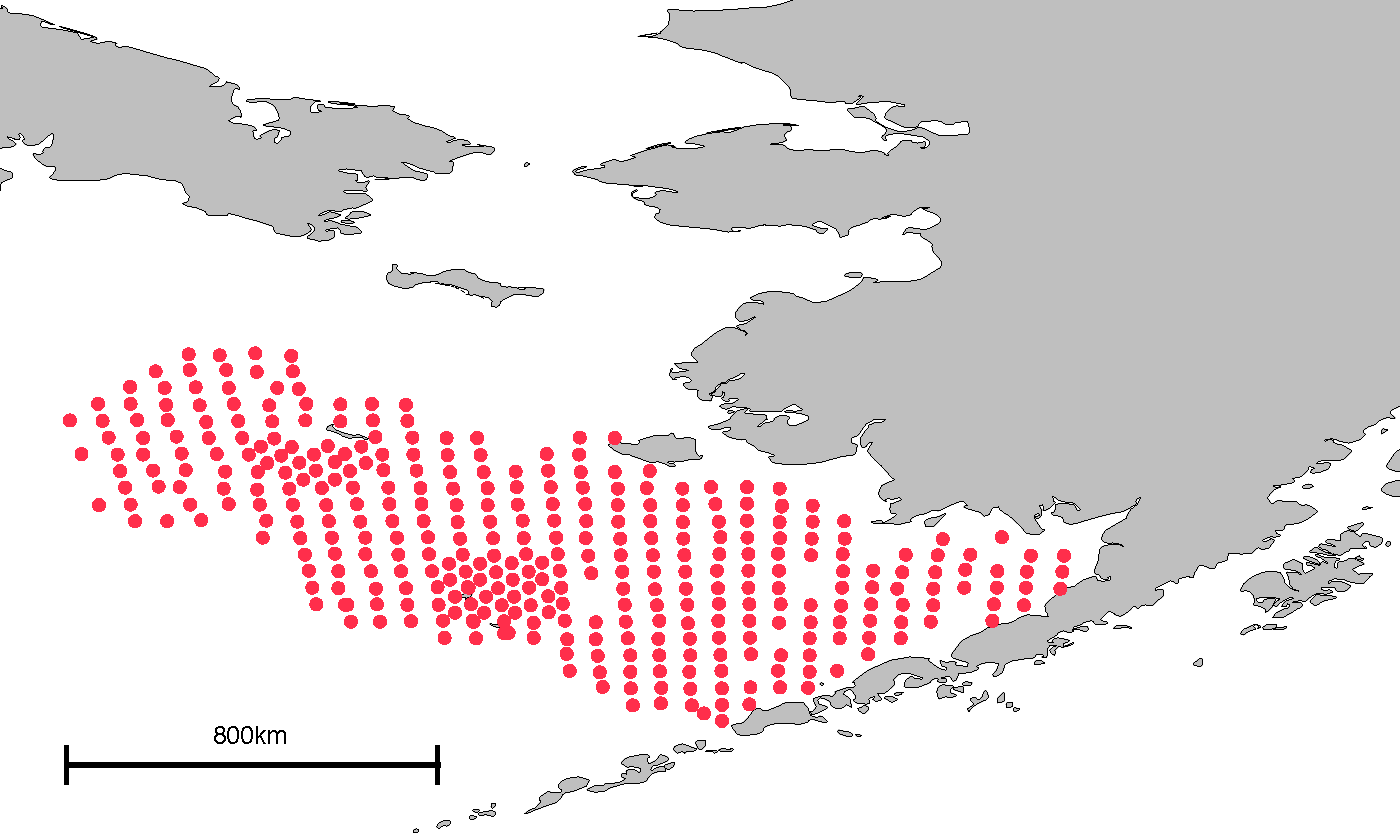
\includegraphics[width=0.85\textwidth]{figs/watercolumns}
  \caption{An oceanographic dataset in the Bering Sea in which samples are distributed along water columns. Each red point represents a (vertical) water column, where samples are collected every 2m.}% 
\label{fig:watercolumns}
\end{figure}
the distribution can be for instance dense vertically (with a sample every 2m in that real-world case) but extremely sparse horizontally (water columns are located at about 35km from each others).


%%%
\subsection{Points to voxels}

The conversion from scattered points to grid is trivial: simply interpolate at regular locations in three dimensions 
\index{interpolation}\marginnote{interpolation}
(which represent the centre of each voxel) and output the results in the appropriate format (grids can be stored in many ways). 
Figure~\ref{fig:r-interpolation} shows the process in two dimensions.
\begin{figure}
  \centering
  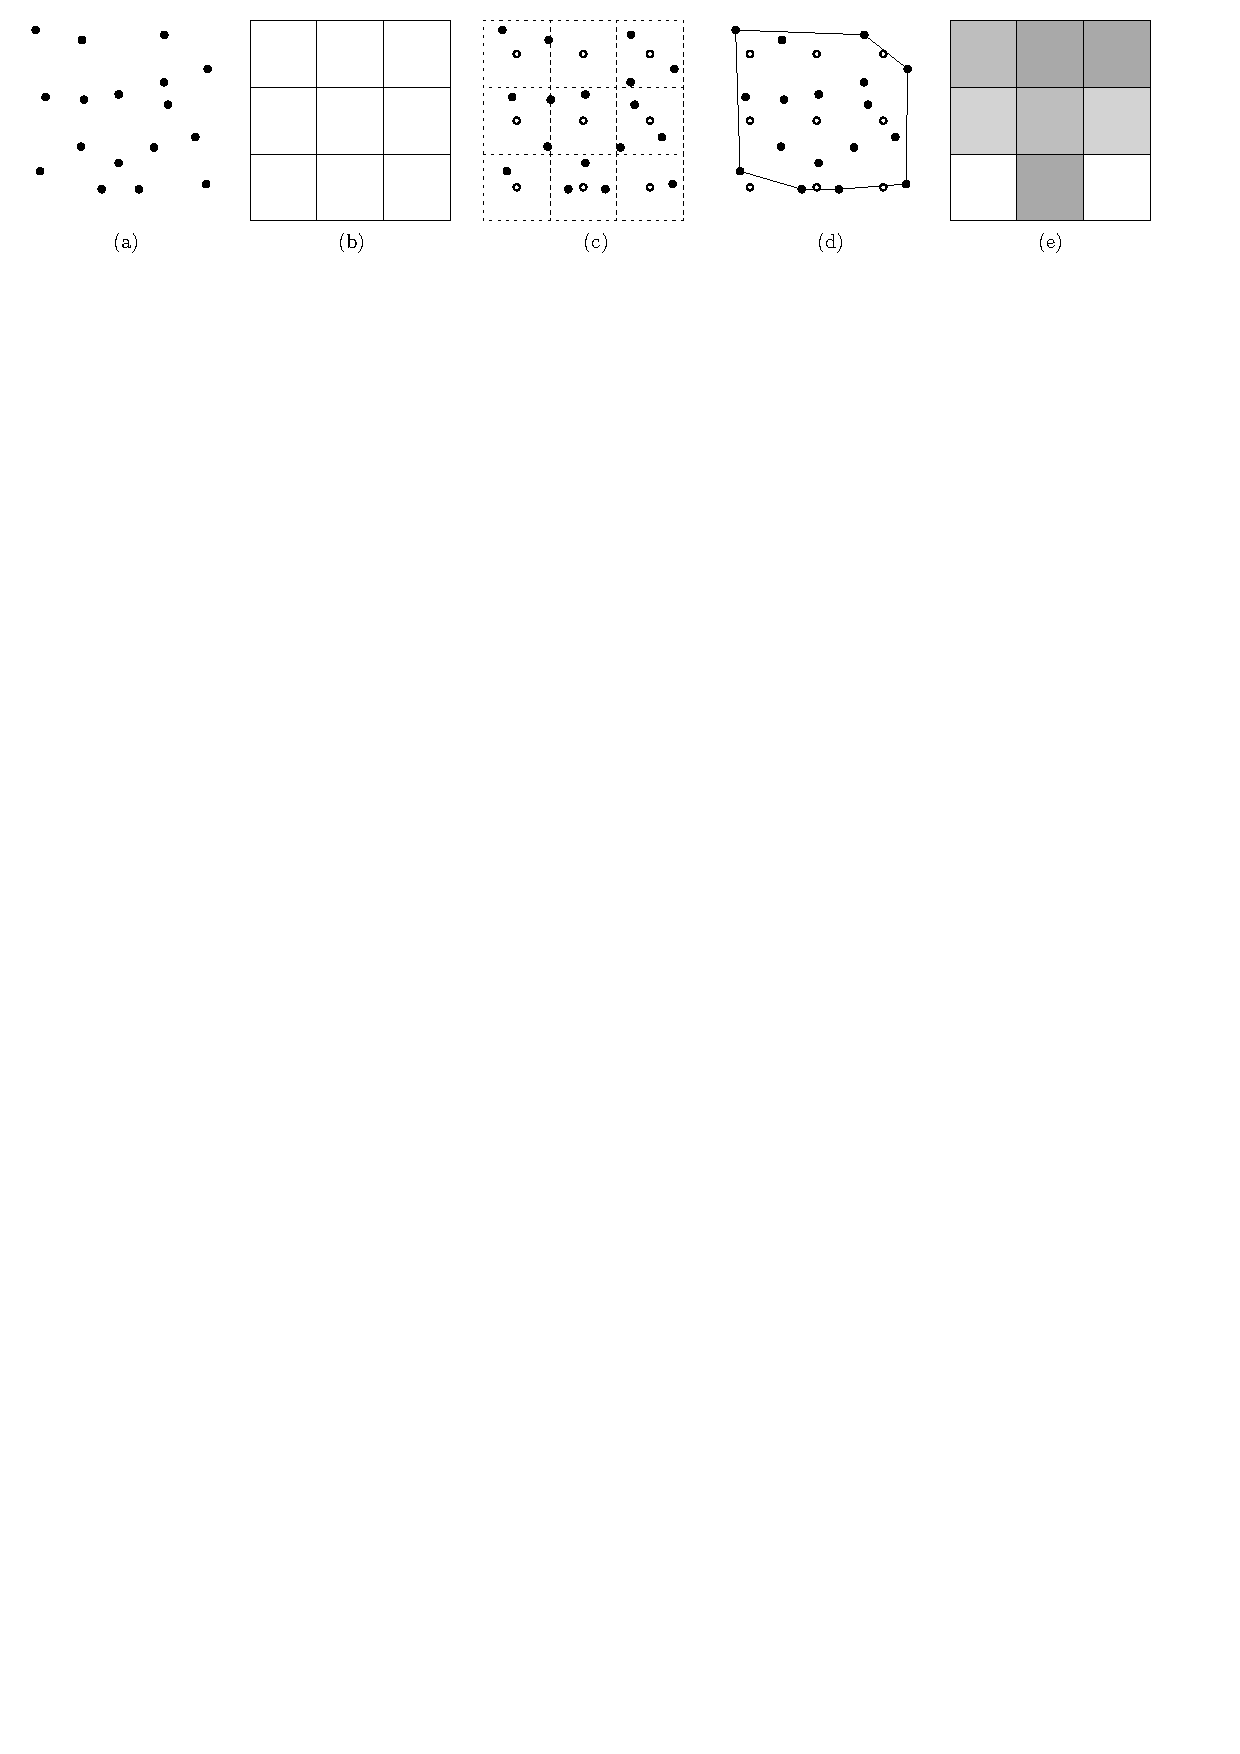
\includegraphics[width=\linewidth]{figs/r-interpolation}
  \caption{\textbf{(a)} input sample points. \textbf{(b)} size/location of output grid. \textbf{(c)} 9 interpolations must be performed (at locations marked with $\circ$): at the middle of each cell. \textbf{(d)} the convex hull of the sample points show that 2 estimations are outside, thus no interpolation. \textbf{(e)} the resulting raster.}%
\label{fig:r-interpolation}
\end{figure}

All the interpolation methods discussed during GEO1015 (Chapters~4 and~5) generalise to three dimensions.
However, it is not obvious that they preserve their properties or are appropriate for geoscientific datasets.

%%%
\paragraph{Nearest neighbour.} 
The method, based on the Voronoi diagram (VD), 
\index{Voronoi diagram}\marginnote{Voronoi diagram}
generalises in a straightforward manner to 3D.
It suffices to build the VD and to identify inside which cell the interpolation point lies.
The VD can be bypassed if a three-dimensional $k$d-tree is used.


%%%
\paragraph{Inverse distance weighting (\textbf{IDW}).}
The generalisation of this method to three dimensions is straightforward: a searching \emph{sphere} with a given radius is used. 
The same problems with the one-dimensionality of the method (the value for the search radius) will be even worse because the search must be performed in one more dimension. 
The method has too many problems to be considered  has a viable solution for fields as found in geosciences: the interpolant is not guaranteed to be continuous, especially when the dataset has an anisotropic distribution (and anisotropy is very frequent in 3D samples, see Lesson~2.2), and the criterion has to be selected carefully by the user.
Note that the implementation problems are also similar to the ones encountered with the previous method, and an auxiliary data structure must be used to avoid testing all the points in a dataset.


%%%
\paragraph{Linear interpolation in tetrahedra.}
This is the generalisation of the popular linear interpolation in TINs where the tetrahedra of the Delaunay tetrahedralisation (DT) are used. 
The barycentric coordinates can be used to linearly interpolate inside a tetrahedron, as shown in Figure~\ref{fig:barycentric} the volumes of 4 tetrahedra are used (instead of the area for the 2D case.)
\begin{marginfigure}
  \centering
  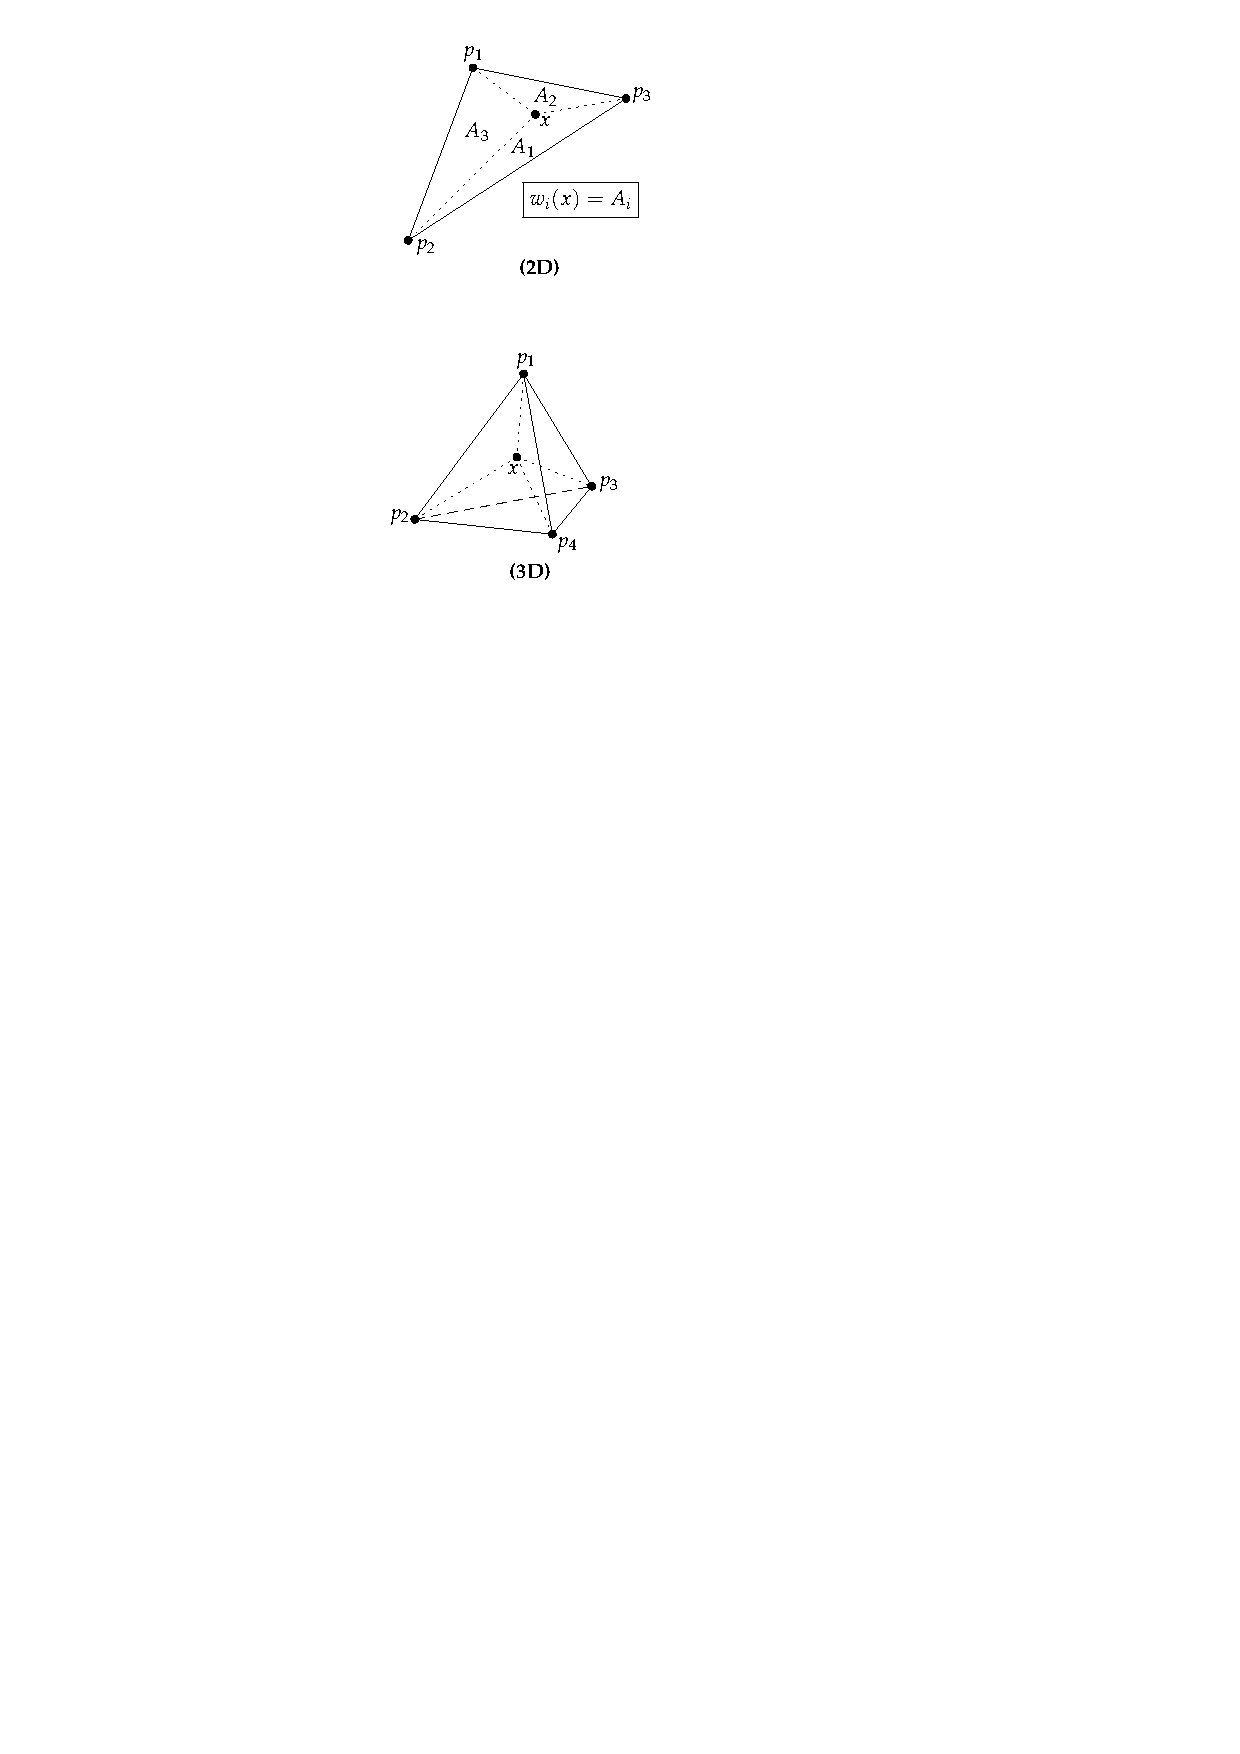
\includegraphics[width=0.9\textwidth]{figs/barycentric}
  \caption{Barycentric coordinates in two and three dimensions. $A_i$ represents the area of the triangle formed by $x$ and one edge.}% 
\label{fig:barycentric}
\end{marginfigure}

The volume of a $d$-simplex $\sigma$ is easily computed:
\begin{equation}
vol(\sigma) = \frac{1}{d \, !} \left| \,  
                            \det \, \left( 
                                  \begin{array}{ccc}
                                    v^{0} & \cdots & v^{d} \\
                                    1     & \cdots & 1 \\
                                  \end{array}
                                \right)
                        \right|
\end{equation}  
where $v^{i}$ is a $d$-dimensional vector representing the coordinates of a vertex and $\det()$ is the determinant of the matrix. 

As explained above, finding tetrahedra having a good shape is not as easy as in two dimensions, and the presence of slivers yield bad results for the interpolation process. 
To be used in practice, the shape of the tetrahedra is usually improved with techniques involving the insertion of new points and/or applying flips.


%%%
\paragraph{Natural neighbour interpolation.}
The theory of this method also generalises in a straightforward manner to 3D.
Instead of having stolen areas, we have stolen \emph{volumes} between the Voronoi cells.
However, although the concepts behind the method are simple and easy to understand, its implementation for the 3D case is far from being straightforward. 
The main reasons are that it requires the computation of two VDs---one with and one without the interpolation point---and also the computation of volumes of Voronoi cells. 
This involves algorithms for both constructing a VD and deleting a point from it.

The volume of a $d$-dimensional Voronoi cell is computed by decomposing it into $d$-simplices---not necessarily Delaunay simplices---and summing their volumes. 
Triangulating a Voronoi cell is easily performed since it is a convex polyhedron.



%%%
\paragraph{kriging.}
All of the most common kriging varieties generalise to three dimensions without major changes, including simple kriging and ordinary kriging.
In the simplest case, covariance functions, experimental variograms and fitted functions work exactly the same as in 2D but are computed using distances in 3D.

However, the vertical direction has a much weaker correlation than the horizontal directions in many fields, \eg\ temperature, pressure and humidity.
Anisotropy is thus a much more significant factor in 3D and almost always has to be modelled.
A minimal solution is a custom distance function that scales the vertical direction.
A better (but still simple) solution involves computing multiple experimental variograms: two (for the horizontal plane \(x,y\) and for the vertical direction \(z\)) or three (for \(x\), \(y\) and \(z\)).



%%%
\subsection{Voxels to points}

The conversion of a voxel to a set of scattered points is not a simple operation.
Given a three-dimensional grid, it is possible to create one data point at the centre of each voxel.
Notice however that potentially a lot of the neighbouring points will be the same value, and thus a lot of redundancy is stored.

%

A better approach to this problem is to consider it as a simplification problem.
Given a set $S$ of points in $\mathbb{R}^3$ representing a field $f$ (where each point $p$ in $S$ as an attribute $a$ attached to itself), the aim is to find a subset $R$ of $S$ which will approximate $f$ as accurately as possible, using as few points as possible. 
The subset $R$ will contain the `important' points of $S$, \ie\ a point $p$ is important when $a$ at location $p$ can not be accurately estimated by using the neighbours of $p$.

%

The two algorithms described in the GEO1015 book (Section~8.3) can in theory be generalised; Figure~\ref{fig:meshsimplification} shows the idea for the 1D case.
\begin{figure}
  \centering
  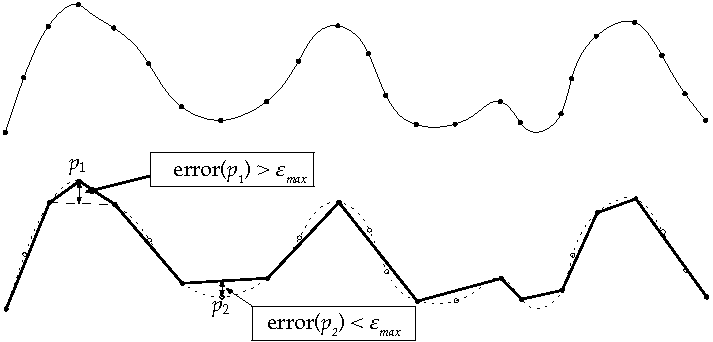
\includegraphics[width=0.85\linewidth]{figs/mesh_simplification}
  \caption{The importance measure of a point can be expressed by its error. When this error is greater than a given threshold $\epsilon_{max}$, the point is kept ($p_1$), else it is discarded ($p_2$).}%
\label{fig:meshsimplification}
\end{figure}
Both strategies (decimation and refinement) can be implemented.

The error associated with each point $p$, denoted error($p$), is calculated by interpolating at location $p$ after $p$ has been temporarily removed from the field, and comparing the value obtained with the real attribute $a$ of $p$, thus error($p) = |a - estimation|$. 
As shown in Figure~\ref{fig:meshsimplification} for a one-dimensional case, when the error is more than $\epsilon_{max}$ then the point must be kept, if it is less then the point can be discarded.

The method for 2D fields in GEO1015 uses linear interpolation in triangles, \ie\ after $p$ has been temporarily deleted from DT($S$), the triangulation is updated and the estimation is obtained with the triangle containing location $p$. 
However, since mentioned earlier, using the DT in 3D for interpolation is not advised (because they contain slivers).
As an alternative, one could use for instance the natural neighbour interpolation, and each error is calculated by interpolating in the field at the location and comparing the real and the estimated value.


%%%
\subsection{Conversion to isosurfaces}

Given a trivariate field $f(x,y,z) = a$, an isosurface is the set of points in space where $f(x,y,z) = a_0$, where $a_0$ is a constant. 
Isosurfaces, also called \emph{level sets}, are the three-dimensional analogous concept to isolines (also called contour lines), which have been traditionally used to represent the elevation in topographic maps. 
Figure~\ref{fig:isosurface} shows one concrete example.
\begin{figure}*
  \centering
  \begin{subfigure}[b]{0.3\linewidth}
    \centering
    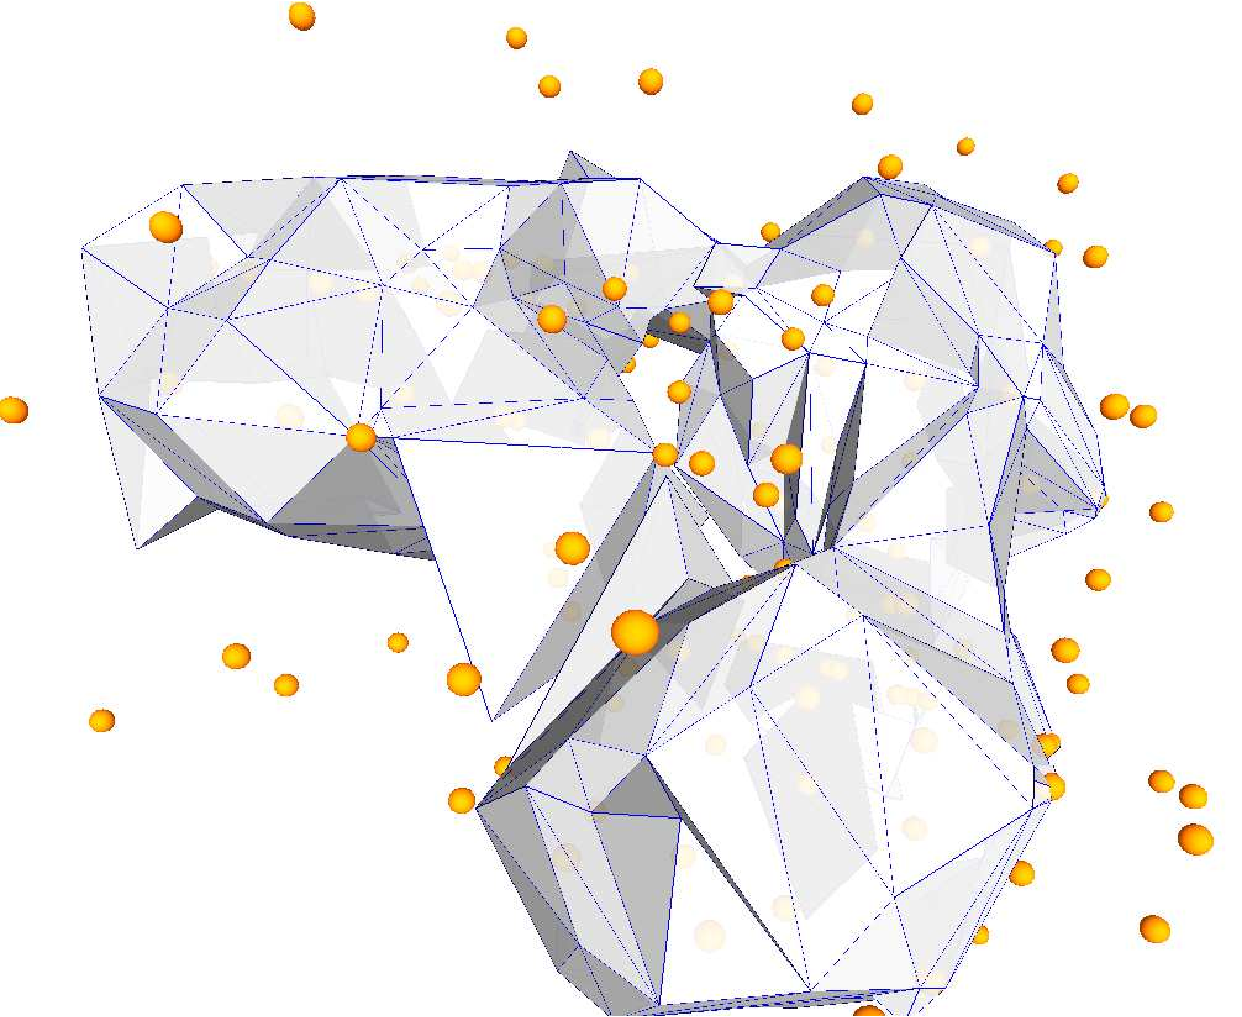
\includegraphics[width=\textwidth]{figs/isosurface2}
    \caption{}
  \end{subfigure}%
  \quad
  \begin{subfigure}[b]{0.3\linewidth}
    \centering
    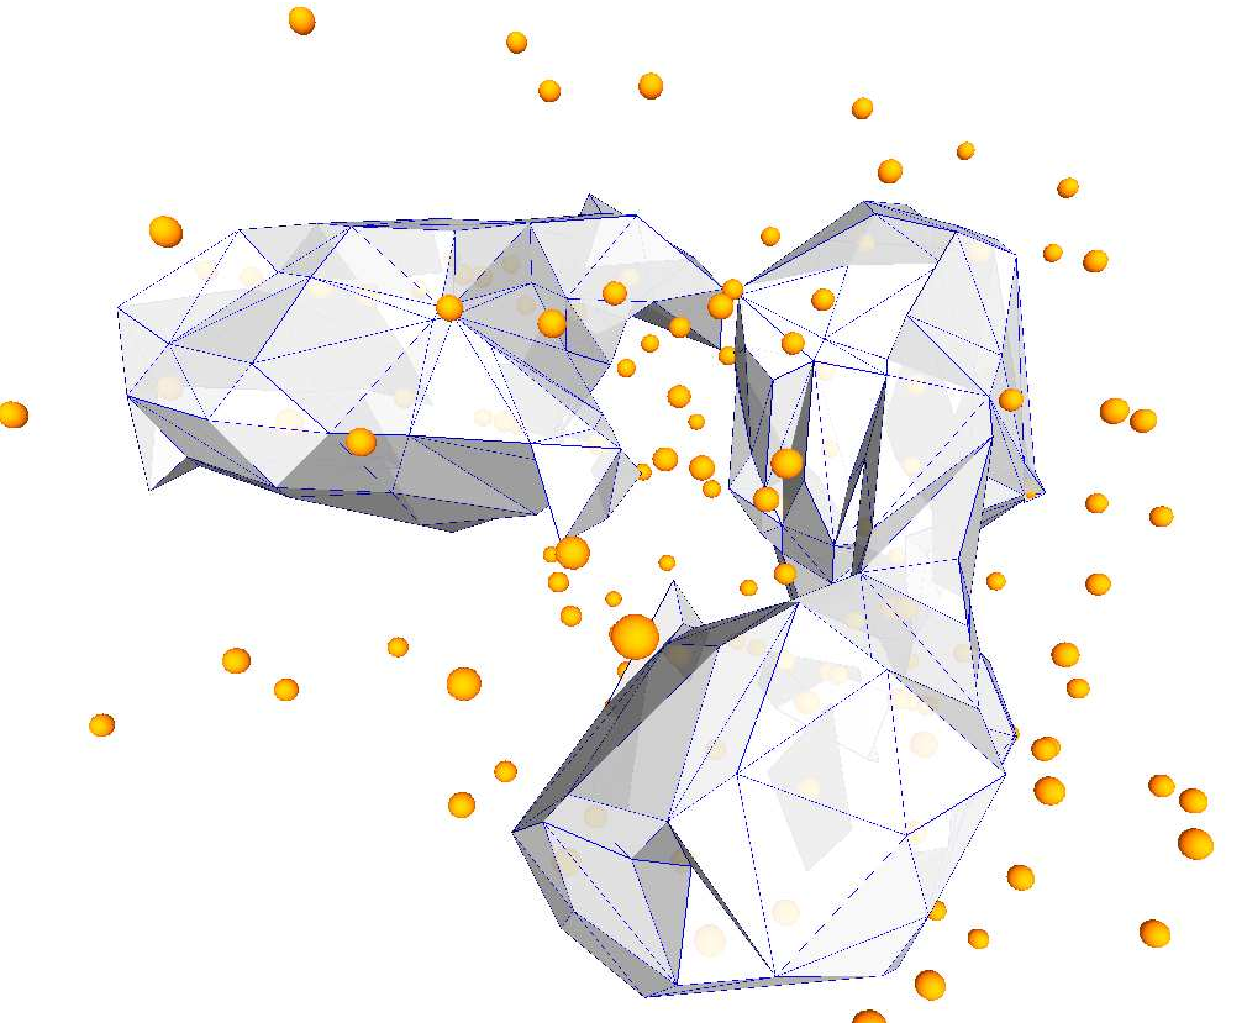
\includegraphics[width=\textwidth]{figs/isosurface25}
    \caption{}
  \end{subfigure}
  \quad
  \begin{subfigure}[b]{0.3\linewidth}
    \centering
    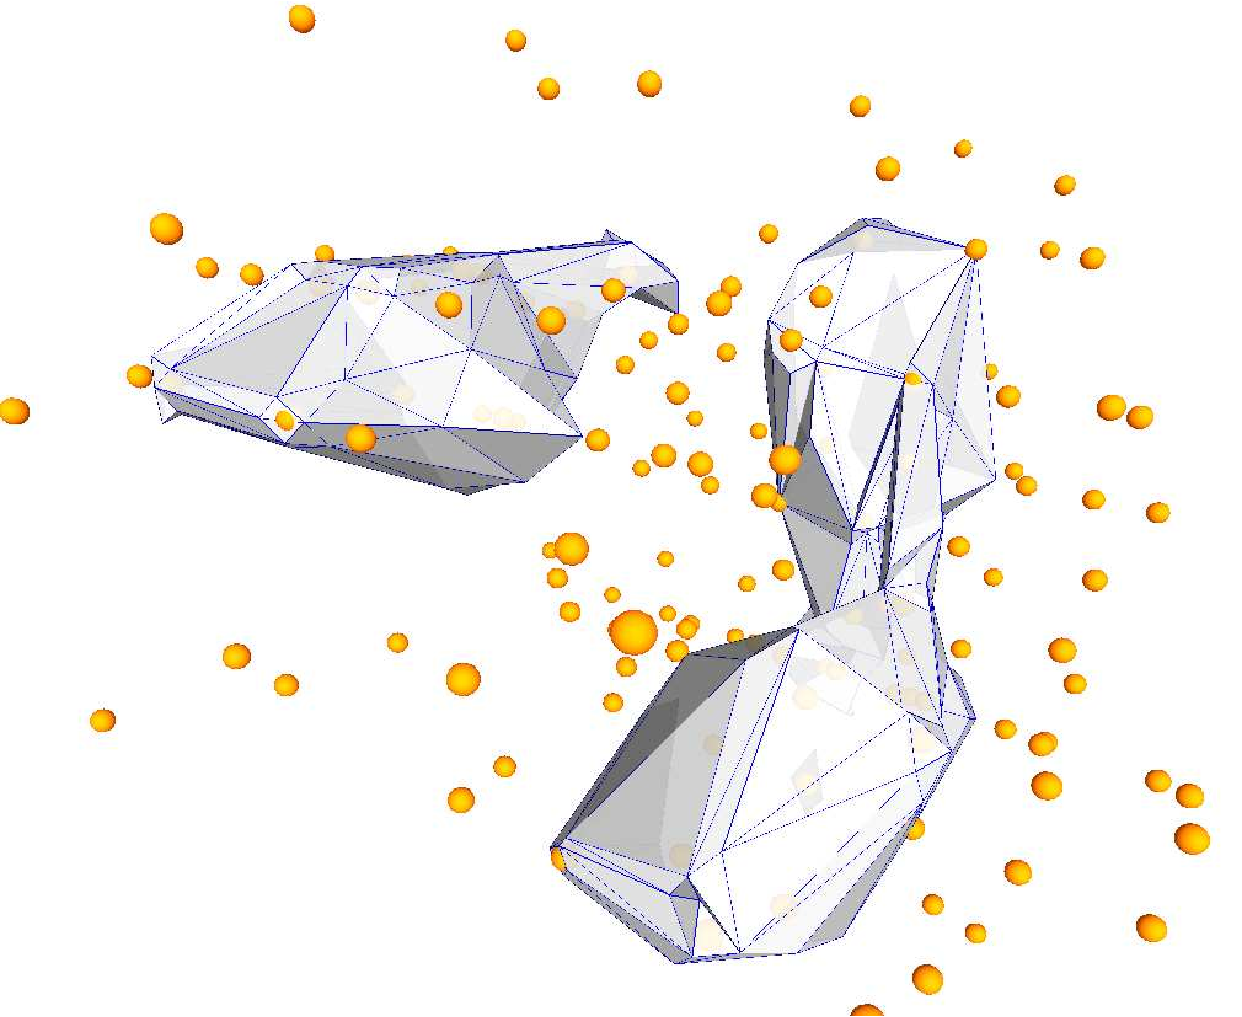
\includegraphics[width=\textwidth]{figs/isosurface3}
    \caption{}
  \end{subfigure}
\caption{An example of an oceanographic dataset where each point has the temperature of the water, and three isosurface extracted (for a value of respectively 2.0, 2.5 and 3.5) from this dataset.}%
\label{fig:isosurface}
\end{figure}*

%

In two dimensions, isolines are usually extracted directly from a TIN or a regular grid. 
The idea is to compute the intersection between the level value (\eg\ 200m) and the terrain, represented for instance with a TIN\@. 
Each triangle is scanned and segment lines are extracted to form an approximation of an isoline.

%

In three dimensions, for a trivariate field, the same idea can be used to extract surfaces.

%

\paragraph{From voxels: Marching Cubes.} 
The principal and most known algorithm for extracting an isosurface form a voxel dataset is the \emph{Marching Cu\-bes}. 
The isosurface is computed by finding the intersections between the isosurface and each voxel/cube of the representation. 
Linear interpolation is used along the edges of each cube to extract `polygonal patches' of the isosurface. 
There exist 256 different cases for the intersection of a surface with a cube (considering that the value of each of the eight vertices of a cube is `above' of `under' the threshold), although if we consider the symmetry in a cube that comes down to only 15 cases. 
The major problem with the marching cubes algorithm is that the isosurface may contain `holes' or `cracks' when a cube is formed by certain configurations of above and under vertices. 
The ambiguities are shown in Figure~\ref{fig:isosurface_ambiguity} for the two-dimensional case when two vertices are above the threshold, and two under, and they form a `saddle'.
\begin{figure}
  \centering
  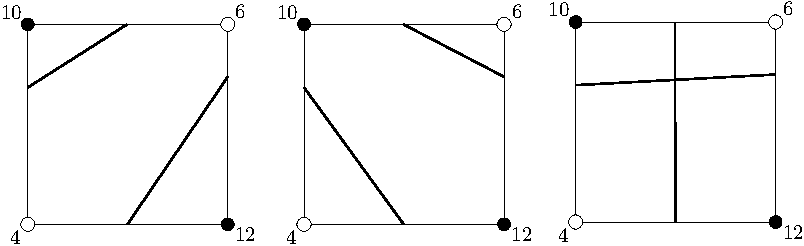
\includegraphics[width=0.7\textwidth]{figs/isosurface_ambiguity}
  \caption{Ambiguous extraction of an isoline where the attribute is 8.}% 
\label{fig:isosurface_ambiguity}
\end{figure}
The three-dimensional case is similar, with many more cases possible. 

%

\paragraph{From tetrahedral mesh: Marching Tetrahedra.} 
Although it is possible to fix the ambiguities, as is the case in two dimensions, the simplest solution is to subdivide each cell into simplices (cubes into tetrahedra in 3D). 
The so-called \emph{Marching Tetrahedra} algorithm is very simple: each tetrahedron is tested for the intersection with the isosurface, and triangular faces are extracted from the tetrahedra by linear interpolation on the edges. 
The resulting isosurface is guaranteed to be topologically consistent (\ie\ will not contain holes), except at the border of the dataset. 
But again, if a big tetrahedron is used where the vertices are assigned to a value lower than the minimum value of the field, then all the isosurfaces extracted are guaranteed to be `watertight'. 
The nice thing about the algorithm is that only three cases for the intersection of the isosurface and a tetrahedron can arise:
\begin{enumerate}
  \item the four vertices have a higher (or lower) value. No intersection.
  \item one vertex has a higher (or lower) value, hence the three others have a lower (or higher) value. Three intersections are thus defined, and a triangular face is extracted. See Figure~\ref{fig:isosurface_3cases}(a) on the left.
  \item two vertices have a higher (or lower) value and the others have a lower (or higher) value. Four intersections are thus defined. To ensure that triangular faces are extracted (better output for graphics cards), the polygon can be split into two triangles, with an arbitrary diagonal. See Figure~\ref{fig:isosurface_3cases}(a) on the right.
\end{enumerate}
\begin{figure}
  \centering
  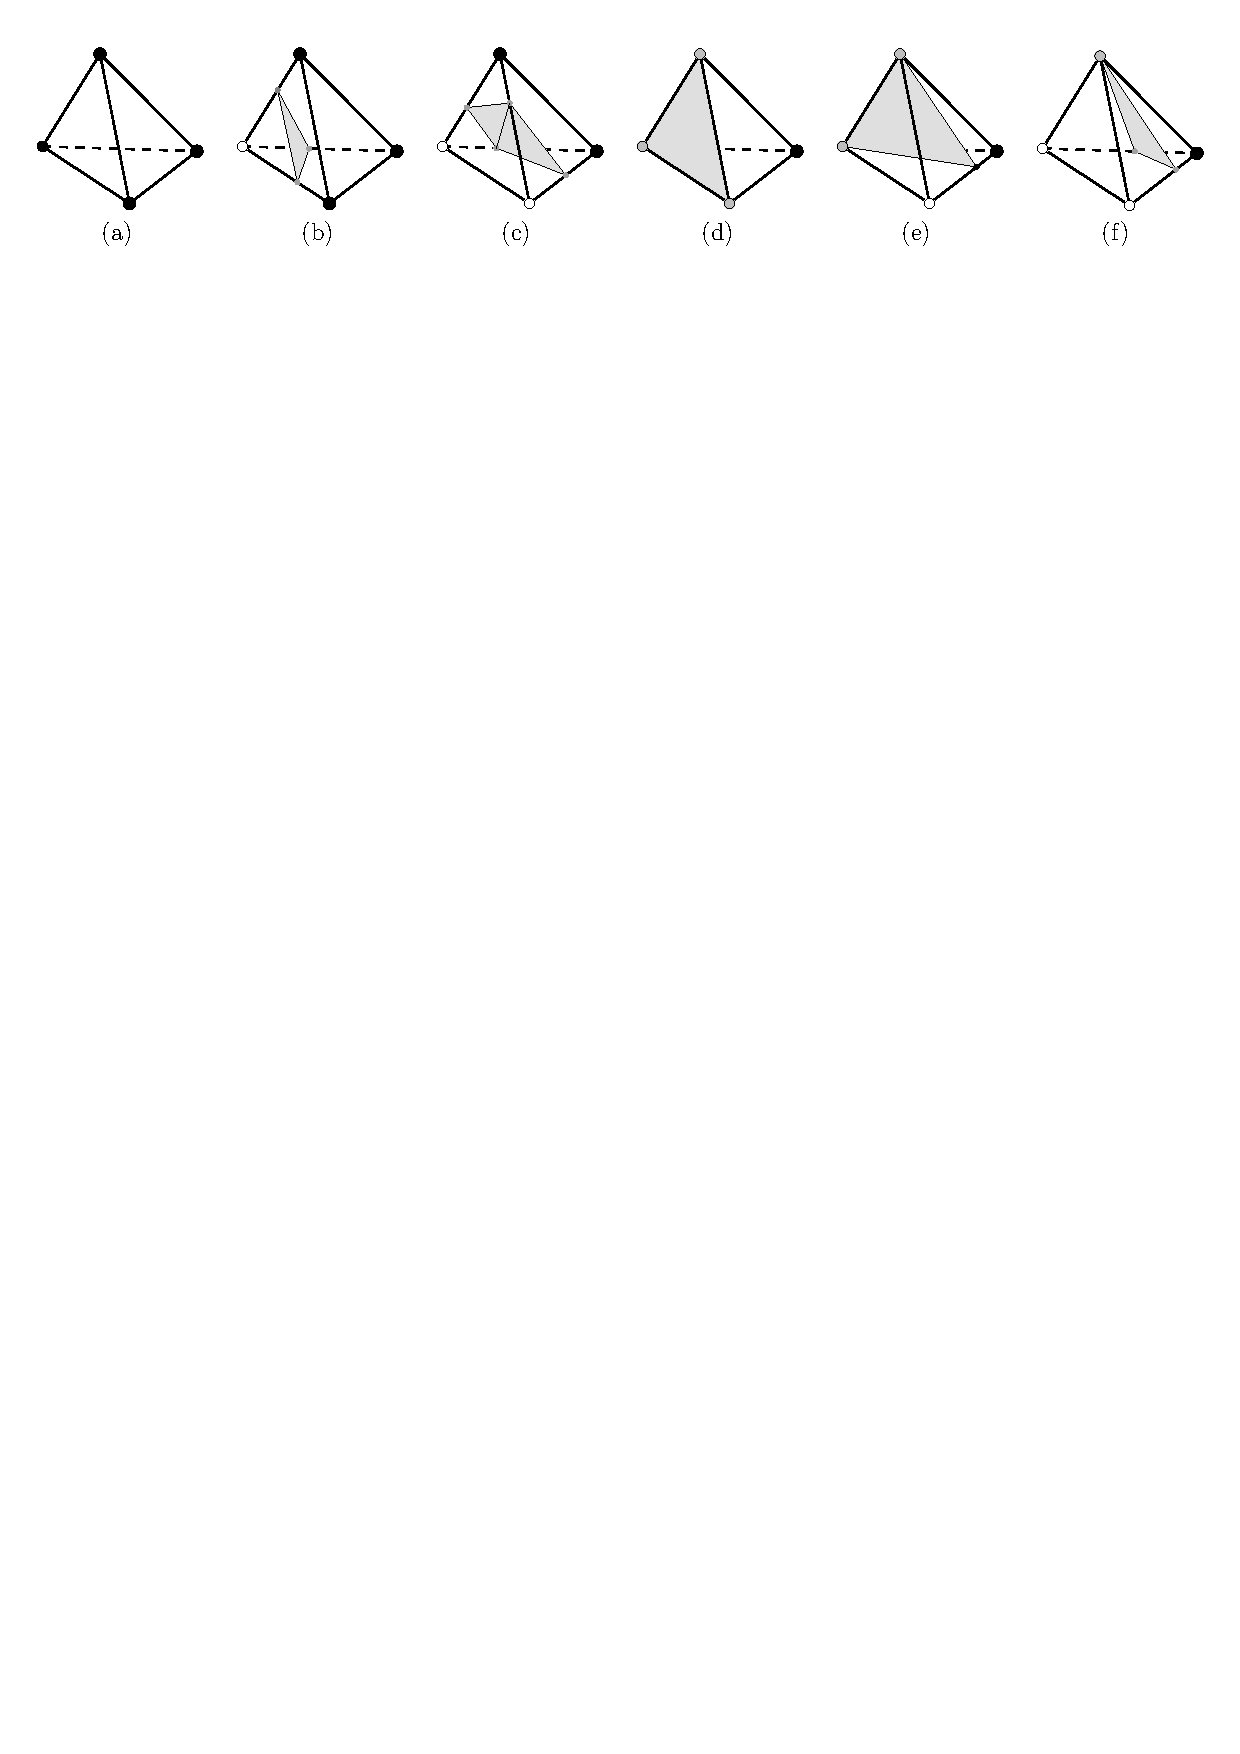
\includegraphics[width=1.0\textwidth]{figs/isosurface_3cases}
  \caption{\textbf{(a)} Two cases for the intersection of an isosurface and a tetrahedron: either 3 or 4 intersections. \textbf{(b)} Three cases when some vertices (the grey ones) have exactly the same value as the isosurface.}% 
\label{fig:isosurface_3cases}
\end{figure}
The only degenerate cases possible are when one or more vertices have exactly the same value as the isosurface. 
These cases are handled very easily, and the intersection is simply assumed to be at the vertices themselves (see Figure~\ref{fig:isosurface_3cases}(b)). 
Notice that the case when three vertices have exactly the same value, then the complete face of the tetrahedron must be extracted to ensure topological consistency.



%%%
%
\section{Conversions for objects}


%%%
\subsection{Points to b-rep}

In the context of the built environment, this would most likely mean that from a point cloud, a LoD2 model of the buildings, and eventually of other objects such as trees and bridges, are reconstructed.

See Lesson~2.1.

%%%
\subsection{Points/surfaces/volumes to voxels}

The conversions of points, curves, surfaces and volumes to voxels are covered in Lesson~3.1.


%%%
\subsection{b-rep to mesh}

For the purposes of this lesson, a \emph{mesh} is a collection of simplices that define the (3D) shape of an object (\eg\ a building, a tree, or a bridge).

If we take the 3D model of a building (say BK-City, see Figure~\ref{fig:bk-mesh}), 
\begin{figure}
  \centering
  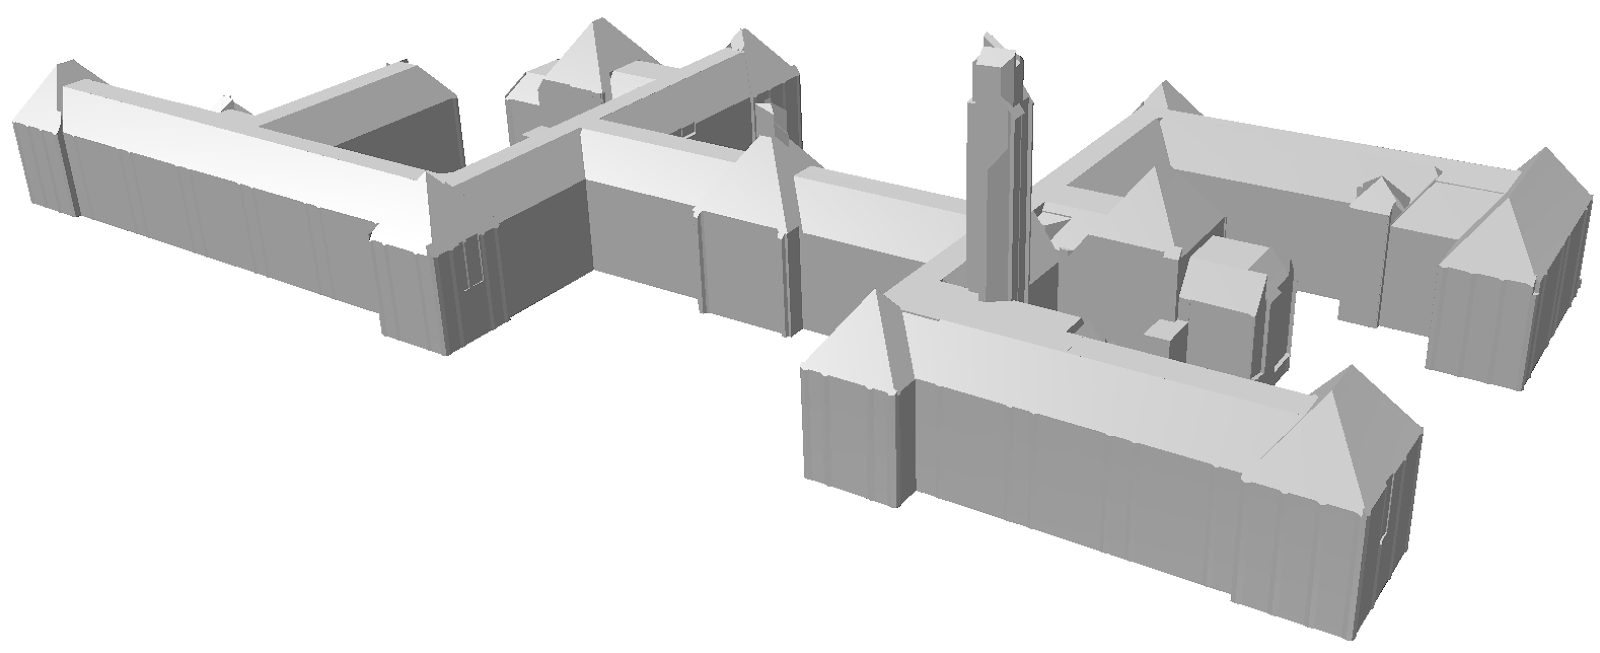
\includegraphics[width=0.5\linewidth]{figs/bk-mesh}
  \caption{b-rep model of BK-City, from Lesson~2.1}%
\label{fig:bk-mesh}
\end{figure}
this model is formed of several planar faces (hopefully) forming a closed 2-manifold.

In practice, if someone wants the mesh of this b-rep, it could mean two different structures:
\begin{description}
  \item[2D triangulation of each surface:] the constrained Delaunay triangulation, or simply an arbitrary constrained triangulation, for each of the polygon can be created. These are independently performed for each surface, and involve transforming the 3D coordinate of the vertices of the surface to a 2D system; this coordinate system is on the plane defined by the surface. Notice that this assumes that all input surfaces of the b-rep are planar, if it is not the case then finding a projection that preserves the topology of the polygon might not be possible.
  \item[tetrahedralisation of the volume defined by the surfaces] the constrained tetrahedralisation of the volume defined by the b-rep; see Section~5 of the Lesson~2.2.
\end{description}

Figure~\ref{fig:meshing} shows one example,
\begin{figure}
  \centering
  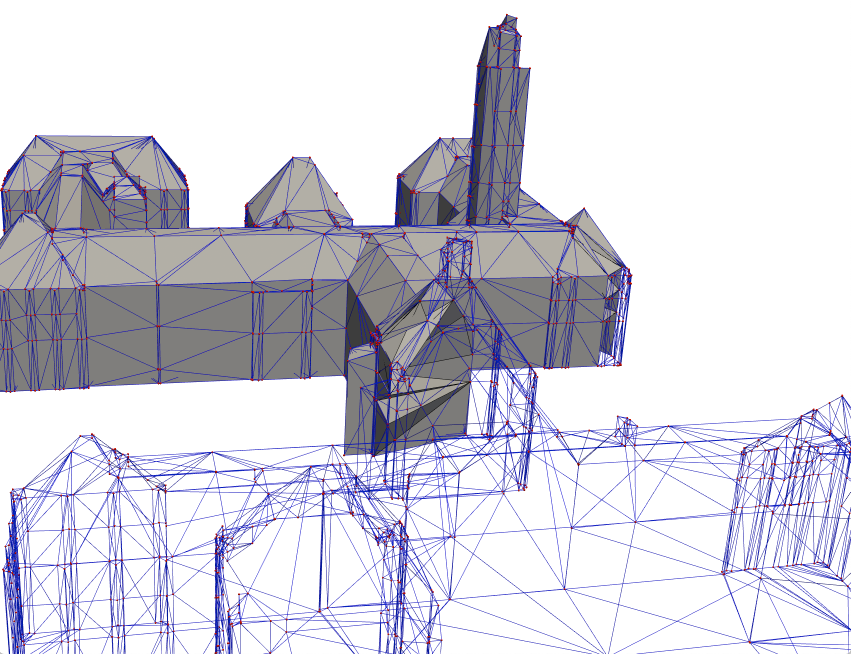
\includegraphics[width=0.65\linewidth]{figs/mesh1}
  \caption{BK-City LoD2 b-rep tetrahedralised.}%
\label{fig:meshing}
\end{figure}
notice that the whole 2-manifold is tetrahedralised, but here only some tetrahedra (in grey) are shown. 
The surfaces of the b-rep also get meshed (each surface is triangulated) in the same process.


%%%
\subsection{IFC to/from CityGML}

The conversion between IFC and the CityGML data model (in either direction) is a very actual topic (many organisation would like to be able to realise it) but it is also riddled with problems caused by the differences in semantics, in data formats, and in the way geometries are modelled.
Automatic conversion with commercial software, \eg\ FME or ArcGIS, will often ``work'', but because of the complexity of some formats, information will often be lost in the conversion. 
Be aware.

The following scientific paper summarises the issues and proposes one solution. 
This solution is (mostly) based on the methods and algorithms we have studied so far in this course.

It should be noticed that this paper is a summary of the MSc thesis of Sjors Donkers, who studied MSc Geomatics in 2014--2015.
This MSc thesis gives you an idea of what a (very good) thesis should look like, in content and in scope.

\begin{kaobox}[frametitle=\faExternalLink\ To read or to watch.]
  \fullcite{Donkers16}
  \\ \\
  PDF: \url{https://3d.bk.tudelft.nl/hledoux/pdfs/16_tgis_ifcitygml.pdf}
  \\ \\
  Full MSc thesis: \url{http://resolver.tudelft.nl/uuid:31380219-f8e8-4c66-a2dc-548c3680bb8d}
\end{kaobox}

%%%
%
\section{Notes and comments}

\citet{Lorensen87} first describe the Marching Cubes algorithm to extract isosurfaces from voxels.
% Although \citet{Wilhems90} describe various methods to fix the ambiguities, as is the case in two dimensions, the simplest solution is to subdivide the cubes into tetrahedra.

%%%
%
\section{Exercises}

\begin{enumerate}
  \item Converting samples points to voxels require totally different algorithm if the samples point represent a field or an object. Discuss why.
  \item If the b-rep model of BK-city contains intersecting surfaces and has gaps/holes, will it be possible to mesh the model?
  \item For terrains, linear interpolation in a TIN is very popular and used. Why is it less popular for trivariate fields?
  \item It is stated in the lesson that ``Triangulating a Voronoi cell is easily performed since it is a convex polyhedron.''. Explain one method.
  \item In the methodology of \citet{Donkers16}, why are the dilation and erosion operators used? Are they always necessary? Can you think of a simple dataset where they could be skipped?
\end{enumerate}
